\documentclass[a4paper, 11pt]{article}

\usepackage[top=3cm, left=2cm, text={17cm,24cm}]{geometry}
\usepackage[utf8]{inputenc}
\usepackage[czech]{babel}
\usepackage{times}
\usepackage{multirow}
\usepackage{amsmath}
\usepackage{cprotect}
\usepackage{graphics}
\usepackage[czech, ruled, linesnumbered, noline, longend]{algorithm2e}
\usepackage{pdflscape}
\usepackage{tikz}


\begin{document}
\begin{titlepage}
\begin{center}
\textsc{\Huge{Vysoké učení technické v Brně\\[0,3em]}
{\huge{Fakulta informačních technologií}}}\\
\vspace{\stretch{0.382}}
{\LARGE Typografie a publikování -- 3. projekt}\\[0,3em]
{\Huge{Tabulky a obrázky}}\\
\vspace{\stretch{0.618}}
{\Large 13. března 2020 \hfill Richard Klem}
\end{center}
\end{titlepage}
\section{Úvodní strana}
\noindent Název práce umístěte do zlatého řezu a nezapomeňte uvést dnešní datum a vaše jméno a příjmení.
\section{Tabulky}
Pro sázení tabulek můžeme použít buď prostředí \verb|tabbing| nebo prostředí \verb|tabular|.
\subsection{Prostředí \texttt{tabbing}}
Při použití \verb|tabbing| vypadá tabulka následovně:
\begin{tabbing}
Vodní melouny\quad \= \textbf{Cena}\quad \= \textbf{Množství}\kill
\textbf{Ovoce} \> \textbf{Cena} \> \textbf{Množství}\\
Jablka    \> 25,90     \> 3 kg\\
Hrušky    \> 27,40     \> 2,5kg\\
Vodní melouny    \> 35,--     \> 1 kus\\
\end{tabbing}

\noindent Toto prostředí se dá také použít pro sázení algoritmů, ovšem vhodnější je použít 
prostředí \verb|algorithm| nebo \verb|algorithm2e| (viz sekce \ref{section:Algoritmy}).
\subsection{Prostředí \texttt{tabular}}
\noindent Další možností, jak vytvořit tabulku, je použít prostředí tabular. Tabulky pak budou vypadat takto
\cprotect\footnote{Kdyby byl problem s\verb| cline,| zkuste se podívat třeba sem: 
http://www.abclinuxu.cz/tex/poradna/show/325037.}:
\bigskip
\begin{table}[h]
\catcode`\-=12
\centering
\begin{tabular}{|c|c|c|}
\hline
\textbf{}     & \multicolumn{2}{c|}{Cena} \\ \cline{2-3} 
\textbf{Měna} & nákup       & prodej      \\ \hline
EUR           & 25,475      & 27,045      \\
GBP           & 28,835      & 30,705      \\
USD           & 22,943      & 24,357      \\ \hline
\end{tabular}
\caption{Tabulka kurzů k dnešnímu dni}
\label{tab:meny}
\end{table}
\bigskip
\begin{table}[h]
    \centering
    \begin{tabular}{|c|c|}
        \hline
        $A$              & $\neg A$    \\ \hline
        \textbf{P} & N \\ \hline
        \textbf{O} & O \\ \hline
        \textbf{X} & X \\ \hline
        \textbf{N} & P \\ \hline
    \end{tabular}
    \catcode`\-=12
    \begin{tabular}{|c|c|c|c|c|c|}
        \hline
        \multicolumn{2}{|c|}{\multirow{2}{*}{$A \wedge B$}} & \multicolumn{4}{c|}{B}                            \\ \cline{3-6} 
        \multicolumn{2}{|c|}{}                     & \textbf{P} & \textbf{O} & \textbf{X} & \textbf{N} \\ \hline
        \multirow{4}{*}{A}       & \textbf{P}      & P          & O          & X          & N          \\ \cline{2-6} 
                                 & \textbf{O}      & O          & O          & N          & N          \\ \cline{2-6} 
                                 & \textbf{X}      & X          & N          & X          & N          \\ \cline{2-6} 
                                 & \textbf{N}      & N          & N          & N          & N          \\ \hline
    \end{tabular}
    \catcode`\-=12
    \begin{tabular}{|c|c|c|c|c|c|}
        \hline
        \multicolumn{2}{|c|}{\multirow{2}{*}{$A \vee B$}} & \multicolumn{4}{c|}{B}                            \\ \cline{3-6} 
        \multicolumn{2}{|c|}{}                     & \textbf{P} & \textbf{O} & \textbf{X} & \textbf{N} \\ \hline
        \multirow{4}{*}{A}       & \textbf{P}      & P          & P          & P          & P          \\ \cline{2-6} 
                                 & \textbf{O}      & P          & O          & P          & O          \\ \cline{2-6} 
                                 & \textbf{X}      & P          & P          & X          & X          \\ \cline{2-6} 
                                 & \textbf{N}      & P          & O          & X          & N          \\ \hline
    \end{tabular}
    \catcode`\-=12
    \begin{tabular}{|c|c|c|c|c|c|}
        \hline
        \multicolumn{2}{|c|}{\multirow{2}{*}{$A \rightarrow B$}} & \multicolumn{4}{c|}{B}                            \\ \cline{3-6} 
        \multicolumn{2}{|c|}{}                     & \textbf{P} & \textbf{O} & \textbf{X} & \textbf{N} \\ \hline
        \multirow{4}{*}{A}       & \textbf{P}      & P          & O          & X          & N          \\ \cline{2-6} 
                                 & \textbf{O}      & P          & O          & P          & O          \\ \cline{2-6} 
                                 & \textbf{X}      & P          & P          & X          & X          \\ \cline{2-6} 
                                 & \textbf{N}      & P          & P          & P          & P          \\ \hline
    \end{tabular}
    \caption{Protože Kleeneho trojhodnotová logika už je \uv{zastaralá}, uvádíme si zde
  příklad čtyřhodnotové logiky}
    \label{tab:logika}
\end{table}
\bigskip
\pagebreak

\section{Algoritmy}
\label{section:Algoritmy}
\noindent Pokud budeme chtít vysázet algoritmus, můžeme použít prostředí\verb| algorithm|\cprotect\footnote{Pro nápovědu, jak zacházet s prostředím\verb| algorithm,| můžeme zkusit tuhle stránku:\\
http://ftp.cstug.cz/pub/tex/CTAN/macros/latex/contrib/algorithms/algorithms.pdf.}
nebo\verb| algorithm2e|\cprotect\footnote{Pro\verb| algorithm2e |zase tuhle:
http://ftp.cstug.cz/pub/tex/CTAN/macros/latex/contrib/algorithm2e/doc/algorithm2e.pdf.}.
Příklad použití prostředí algorithm2e viz Algoritmus \ref{algorithm:algo1}.

\IncMargin{1.5em}
\begin{algorithm}[h]
\caption{\textsc{FastSLAM}}
\label{algorithm:algo1}
%\begin{algorithmic}[1]
\SetNlSty{}{}{:}
    
    \Indm\Indmm
    \KwIn{$(X_{t - 1}, u_t, z_t)$}
    \KwOut{$ X_t$}
    \medskip
    \Indp\Indpp
    $\overline{X_t} = X_t = 0$\\
    \For{$k = 1$ \emph{to} $M$}{
    $x_t^{[k]} = \emph{sample\_motion\_model}(u_t, x_{t - 1}^{[k]})$\\
    $\omega_t^{[k]} = \emph{measurement\_model}(z_t, x_t^{[k]}, m_{t - 1})$\\
    $m_t^{[k]} = updated\_occupancy\_grid(z_t, x_t^{[k]}, m_{t - 1}^{[k]})$\\
    $\overline{X_t} = \overline{X_t} + \langle x_x^{[m]}, \omega_t^{[m]} \rangle$}
    \For{$k = 1$ \emph{to} $M$}{
    $\text{draw } i \text{ with probability} \approx \omega_t^{[i]}$\\
    $\text{add}\, \langle x_x^{[k]}, m_t^{[k]} \rangle \textrm{ to } X_t$}
    \KwRet{$X_t$}
%\end{algorithmic}
\end{algorithm}

\section{Obrázky}
\noindent Do našich článků můžeme samozřejmě vkládat obrázky. Pokud je obrázkem fotografie,
můžeme klidně použít bitmapový soubor. Pokud by to ale mělo být nějaké schéma nebo
něco podobného, je dobrým zvykem takovýto obrázek vytvořit vektorově.
\begin{figure}[h]
    \centering
    \scalebox{0.4}{
    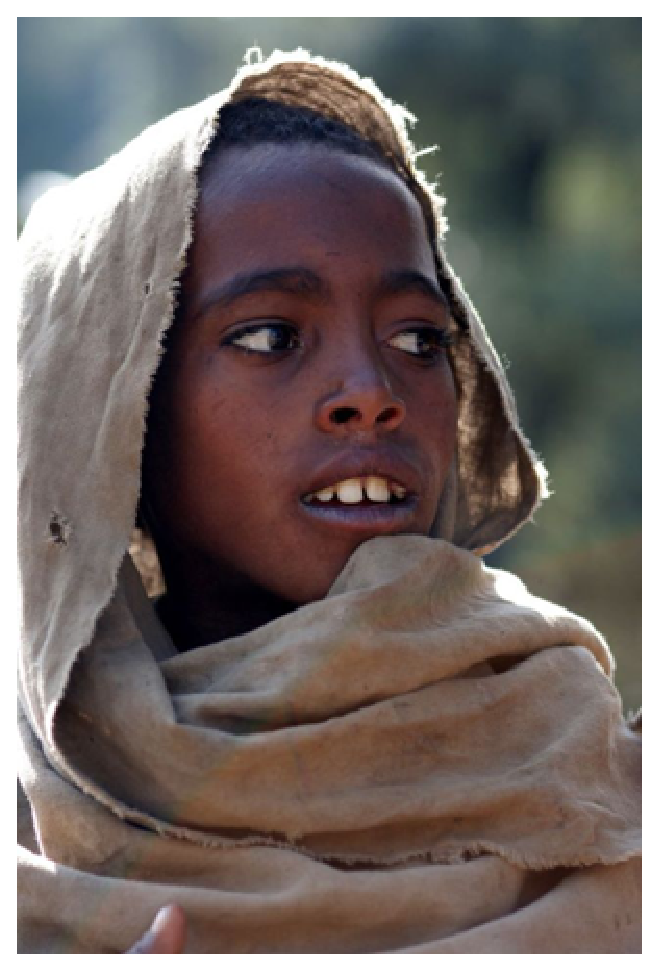
\includegraphics{etiopan.eps}
    \reflectbox{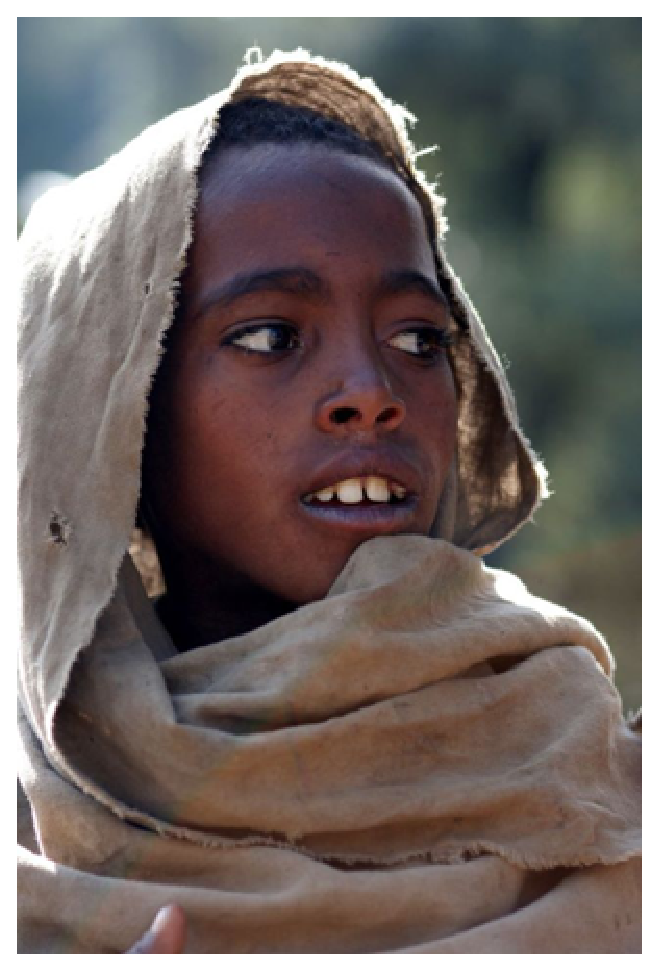
\includegraphics{etiopan.eps}}
    }
    \caption{Malý Etiopánek a jeho bratříček}
    \label{fig:etiopan}
\end{figure}
\newpage
Rozdíl mezi vektorovým\dots
\begin{figure}[h]
    \centering
    \scalebox{0.4}{
    
\includegraphics{oniisan.eps}
    }
    \caption{Vektorový obrázek}
    \label{fig:vektor}
\end{figure}\\[1em]
\dots a bitmapovým obrázkem
\begin{figure}[h]
    \centering
    \scalebox{0.6}{
    
\includegraphics{oniisan2.eps}
    }
    \caption{Bitmapový obrázek}
    \label{fig:bitmap}
\end{figure}\\[1em]
\noindent se projeví například při zvětšení.

Odkazy (nejen ty) na obrázky \ref{fig:etiopan}, \ref{fig:vektor} a \ref{fig:bitmap}, na 
tabulky \ref{tab:meny} a \ref{tab:logika} a také na algoritmus \ref{algorithm:algo1} jsou udělány pomocí 
křížových odkazů. Pak je ovšem potřeba zdrojový soubor přeložit dvakrát.

Vektorové obrázky lze vytvořit i přímo v \LaTeX u, například pomocí prostředí 
\verb|picture|.
\newpage
\begin{landscape}
\begin{figure}
    \centering
    \tikzset{every picture/.style={line width=0.75pt}} %set default line width to 0.75pt        
    \begin{tikzpicture}[x=0.75pt,y=0.75pt,yscale=-1,xscale=1]
    %uncomment if require: \path (0,449); %set diagram left start at 0, and has height of 449
    
    %Shape: Rectangle [id:dp09667141586182337] 
    \draw   (112,318.2) -- (439.3,318.2) -- (439.3,410.2) -- (112,410.2) -- cycle ;
    %Shape: Rectangle [id:dp864829618606054] 
    \draw   (439.3,318.2) -- (532.31,225.48) -- (532.29,317.38) -- (439.28,410.1) -- cycle ;
    %Straight Lines [id:da4825672797522442] 
    \draw    (264.01,227.48) -- (249.5,227.8) ;
    %Shape: Rectangle [id:dp8963150067519137] 
    \draw   (263.81,226.43) -- (472.89,226.43) -- (472.89,285.2) -- (263.81,285.2) -- cycle ;
    %Shape: Rectangle [id:dp35254545968400275] 
    \draw   (472.89,226.43) -- (532.31,167.2) -- (532.3,225.9) -- (472.88,285.13) -- cycle ;
    %Straight Lines [id:da728111388775351] 
    \draw    (263.81,226.43) -- (323.23,167.2) ;
    %Straight Lines [id:da009795771279418553] 
    \draw    (323.23,167.2) -- (532.31,167.2) ;
    %Shape: Rectangle [id:dp34232377227204136] 
    \draw   (143.3,351.2) -- (231,351.2) -- (231,381) -- (143.3,381) -- cycle ;
    %Straight Lines [id:da9610807463363347] 
    \draw    (187.15,351.1) -- (187.15,370.24) -- (187.15,381.1) ;
    %Straight Lines [id:da3775074188886829] 
    \draw    (231.15,366.1) -- (143.15,366.1) ;
    %Shape: Rectangle [id:dp14715214959637213] 
    \draw   (299.3,350.2) -- (387,350.2) -- (387,380) -- (299.3,380) -- cycle ;
    %Straight Lines [id:da6141176038536134] 
    \draw    (343.15,350.1) -- (343.15,380.1) ;
    %Straight Lines [id:da45354292379888594] 
    \draw    (387.15,365.1) -- (299.15,365.1) ;
    %Shape: Rectangle [id:dp677113684117175] 
    \draw   (280.46,242.2) -- (459.99,242.2) -- (459.99,272) -- (280.46,272) -- cycle ;
    %Straight Lines [id:da16291295782312765] 
    \draw    (328.22,241.1) -- (328.22,263.2) -- (328.22,271.1) ;
    %Straight Lines [id:da931710650400758] 
    \draw    (460.3,257.1) -- (280.15,257.1) ;
    %Straight Lines [id:da9169264051814479] 
    \draw    (411.22,242.1) -- (411.22,264.2) -- (411.22,272.1) ;
    %Shape: Rectangle [id:dp5535466119365517] 
    \draw   (483.31,304.16) -- (501.3,286.22) -- (501.29,348.38) -- (483.29,366.32) -- cycle ;
    %Shape: Circle [id:dp6106924989015787] 
    \draw   (498.25,324.21) .. controls (498.84,323.52) and (499.89,322.96) .. (500.58,322.96) .. controls (501.28,322.96) and (501.35,323.52) .. (500.75,324.21) .. controls (500.15,324.91) and (499.11,325.47) .. (498.41,325.47) .. controls (497.72,325.47) and (497.65,324.91) .. (498.25,324.21) -- cycle ;
    %Straight Lines [id:da2773105311766144] 
    \draw    (205.01,203.22) -- (285.5,204) ;
    %Straight Lines [id:da6447265742593009] 
    \draw    (112,318.2) -- (112,295.94) ;
    %Straight Lines [id:da7652552277262128] 
    \draw    (205.75,225.04) -- (205.01,203.22) ;
    %Straight Lines [id:da057032752990445745] 
    \draw    (227,318.2) -- (227,295.94) ;
    %Straight Lines [id:da06104752555051829] 
    \draw    (112,295.94) -- (227,295.94) ;
    %Straight Lines [id:da11019898814173201] 
    \draw    (112,295.94) -- (205.01,203.22) ;
    %Straight Lines [id:da4865108053731906] 
    \draw    (134.5,296.6) -- (170.5,260.6) ;
    %Shape: Cloud [id:dp6761721138106311] 
    \draw   (213.54,79.76) .. controls (213.13,76.9) and (214.48,74.07) .. (217.01,72.46) .. controls (219.55,70.86) and (222.83,70.77) .. (225.45,72.23) .. controls (226.39,70.57) and (228.09,69.42) .. (230.05,69.14) .. controls (232.01,68.85) and (234,69.46) .. (235.42,70.78) .. controls (236.21,69.27) and (237.77,68.26) .. (239.54,68.1) .. controls (241.31,67.94) and (243.04,68.66) .. (244.12,70) .. controls (245.55,68.4) and (247.83,67.73) .. (249.97,68.27) .. controls (252.11,68.82) and (253.73,70.48) .. (254.12,72.54) .. controls (255.88,72.99) and (257.34,74.15) .. (258.13,75.7) .. controls (258.92,77.26) and (258.96,79.06) .. (258.25,80.65) .. controls (259.98,82.78) and (260.38,85.62) .. (259.31,88.11) .. controls (258.24,90.6) and (255.85,92.37) .. (253.04,92.75) .. controls (253.02,95.08) and (251.67,97.23) .. (249.51,98.35) .. controls (247.34,99.48) and (244.7,99.41) .. (242.61,98.17) .. controls (241.72,100.97) and (239.21,103.03) .. (236.16,103.46) .. controls (233.12,103.89) and (230.08,102.61) .. (228.37,100.18) .. controls (226.28,101.38) and (223.76,101.73) .. (221.39,101.14) .. controls (219.02,100.56) and (217,99.09) .. (215.79,97.07) .. controls (213.64,97.31) and (211.57,96.26) .. (210.6,94.44) .. controls (209.63,92.62) and (209.96,90.42) .. (211.43,88.93) .. controls (209.52,87.86) and (208.55,85.75) .. (209.02,83.69) .. controls (209.49,81.62) and (211.29,80.08) .. (213.5,79.87) ; \draw   (211.44,88.93) .. controls (212.34,89.43) and (213.38,89.66) .. (214.42,89.58)(215.79,97.07) .. controls (216.23,97.02) and (216.67,96.91) .. (217.09,96.76)(228.37,100.18) .. controls (228.06,99.74) and (227.79,99.26) .. (227.59,98.75)(242.61,98.17) .. controls (242.77,97.66) and (242.88,97.14) .. (242.93,96.6)(253.04,92.75) .. controls (253.06,90.26) and (251.57,87.98) .. (249.21,86.89)(258.25,80.65) .. controls (257.86,81.5) and (257.28,82.25) .. (256.54,82.85)(254.12,72.54) .. controls (254.19,72.88) and (254.22,73.23) .. (254.21,73.58)(244.12,70) .. controls (243.76,70.4) and (243.46,70.84) .. (243.24,71.32)(235.42,70.78) .. controls (235.23,71.14) and (235.09,71.53) .. (235,71.92)(225.45,72.23) .. controls (226.01,72.54) and (226.53,72.91) .. (226.99,73.34)(213.54,79.76) .. controls (213.6,80.15) and (213.69,80.54) .. (213.81,80.92) ;
    %Shape: Cloud [id:dp9545514759655724] 
    \draw   (521.45,73.67) .. controls (520.79,69.12) and (522.96,64.61) .. (527.03,62.06) .. controls (531.1,59.51) and (536.36,59.37) .. (540.59,61.69) .. controls (542.08,59.05) and (544.82,57.22) .. (547.97,56.76) .. controls (551.12,56.31) and (554.31,57.28) .. (556.59,59.38) .. controls (557.86,56.98) and (560.36,55.37) .. (563.2,55.11) .. controls (566.04,54.86) and (568.82,56.01) .. (570.55,58.14) .. controls (572.85,55.59) and (576.52,54.52) .. (579.95,55.39) .. controls (583.39,56.25) and (585.99,58.9) .. (586.62,62.18) .. controls (589.44,62.9) and (591.79,64.74) .. (593.06,67.22) .. controls (594.33,69.69) and (594.4,72.57) .. (593.25,75.09) .. controls (596.02,78.49) and (596.67,83.01) .. (594.95,86.98) .. controls (593.23,90.94) and (589.4,93.75) .. (584.89,94.36) .. controls (584.86,98.08) and (582.68,101.49) .. (579.21,103.28) .. controls (575.73,105.07) and (571.5,104.96) .. (568.13,102.99) .. controls (566.7,107.45) and (562.67,110.73) .. (557.78,111.41) .. controls (552.89,112.1) and (548.02,110.06) .. (545.27,106.19) .. controls (541.9,108.1) and (537.86,108.65) .. (534.06,107.72) .. controls (530.26,106.79) and (527.01,104.45) .. (525.06,101.24) .. controls (521.62,101.61) and (518.29,99.94) .. (516.73,97.04) .. controls (515.17,94.15) and (515.7,90.64) .. (518.07,88.27) .. controls (515,86.58) and (513.43,83.21) .. (514.19,79.93) .. controls (514.94,76.64) and (517.84,74.19) .. (521.38,73.85) ; \draw   (518.07,88.27) .. controls (519.52,89.08) and (521.19,89.44) .. (522.87,89.31)(525.06,101.24) .. controls (525.78,101.16) and (526.48,100.99) .. (527.16,100.74)(545.27,106.19) .. controls (544.76,105.48) and (544.34,104.72) .. (544.01,103.92)(568.13,102.99) .. controls (568.4,102.18) and (568.57,101.34) .. (568.64,100.5)(584.89,94.36) .. controls (584.92,90.4) and (582.53,86.77) .. (578.73,85.03)(593.25,75.09) .. controls (592.63,76.44) and (591.69,77.64) .. (590.5,78.59)(586.62,62.18) .. controls (586.72,62.73) and (586.77,63.28) .. (586.76,63.83)(570.55,58.14) .. controls (569.98,58.77) and (569.51,59.48) .. (569.15,60.24)(556.59,59.38) .. controls (556.28,59.96) and (556.05,60.57) .. (555.91,61.2)(540.59,61.69) .. controls (541.48,62.18) and (542.31,62.78) .. (543.05,63.45)(521.45,73.67) .. controls (521.54,74.3) and (521.69,74.92) .. (521.88,75.52) ;
    %Shape: Cloud [id:dp6556981795567416] 
    \draw   (371.72,99.49) .. controls (371.38,97.92) and (372.49,96.37) .. (374.58,95.49) .. controls (376.67,94.61) and (379.37,94.56) .. (381.53,95.36) .. controls (382.3,94.45) and (383.7,93.82) .. (385.32,93.66) .. controls (386.94,93.5) and (388.57,93.84) .. (389.74,94.56) .. controls (390.39,93.74) and (391.67,93.18) .. (393.13,93.09) .. controls (394.59,93) and (396.01,93.4) .. (396.9,94.13) .. controls (398.08,93.26) and (399.96,92.89) .. (401.72,93.19) .. controls (403.49,93.48) and (404.82,94.4) .. (405.14,95.53) .. controls (406.59,95.78) and (407.79,96.41) .. (408.44,97.26) .. controls (409.09,98.12) and (409.13,99.11) .. (408.54,99.98) .. controls (409.96,101.15) and (410.3,102.71) .. (409.41,104.07) .. controls (408.53,105.44) and (406.57,106.41) .. (404.25,106.62) .. controls (404.24,107.9) and (403.12,109.08) .. (401.34,109.69) .. controls (399.56,110.31) and (397.39,110.27) .. (395.66,109.6) .. controls (394.93,111.13) and (392.86,112.26) .. (390.35,112.5) .. controls (387.84,112.73) and (385.35,112.03) .. (383.94,110.7) .. controls (382.21,111.36) and (380.14,111.55) .. (378.19,111.22) .. controls (376.24,110.9) and (374.57,110.1) .. (373.57,108.99) .. controls (371.81,109.12) and (370.1,108.54) .. (369.3,107.54) .. controls (368.5,106.55) and (368.77,105.34) .. (369.99,104.52) .. controls (368.41,103.94) and (367.61,102.78) .. (368,101.64) .. controls (368.38,100.51) and (369.87,99.67) .. (371.69,99.55) ; \draw   (369.99,104.52) .. controls (370.73,104.8) and (371.59,104.92) .. (372.45,104.88)(373.57,108.99) .. controls (373.94,108.96) and (374.3,108.91) .. (374.65,108.82)(383.94,110.7) .. controls (383.68,110.45) and (383.46,110.19) .. (383.29,109.92)(395.66,109.6) .. controls (395.8,109.32) and (395.88,109.03) .. (395.92,108.74)(404.25,106.62) .. controls (404.27,105.25) and (403.04,104) .. (401.1,103.4)(408.54,99.98) .. controls (408.22,100.44) and (407.74,100.86) .. (407.13,101.18)(405.14,95.53) .. controls (405.19,95.72) and (405.22,95.91) .. (405.21,96.1)(396.9,94.13) .. controls (396.61,94.35) and (396.36,94.6) .. (396.18,94.86)(389.74,94.56) .. controls (389.58,94.76) and (389.46,94.97) .. (389.39,95.19)(381.53,95.36) .. controls (381.99,95.53) and (382.42,95.73) .. (382.8,95.97)(371.72,99.49) .. controls (371.77,99.7) and (371.84,99.92) .. (371.94,100.13) ;
    %Shape: Moon [id:dp06063489430247326] 
    \draw   (135,97.08) .. controls (112.91,97.08) and (95,81.41) .. (95,62.08) .. controls (95,42.75) and (112.91,27.08) .. (135,27.08) .. controls (123.04,34.07) and (115,47.13) .. (115,62.08) .. controls (115,77.03) and (123.04,90.09) .. (135,97.08) -- cycle ;
    %Shape: Star [id:dp2618520163650737] 
    \draw   (158.62,156.08) -- (161.97,162.33) -- (169.44,163.34) -- (164.03,168.2) -- (165.31,175.07) -- (158.62,171.83) -- (151.93,175.07) -- (153.21,168.2) -- (147.8,163.34) -- (155.28,162.33) -- cycle ;
    %Shape: Star [id:dp34617198448520314] 
    \draw   (325.62,33.08) -- (328.97,39.33) -- (336.44,40.34) -- (331.03,45.2) -- (332.31,52.07) -- (325.62,48.83) -- (318.93,52.07) -- (320.21,45.2) -- (314.8,40.34) -- (322.28,39.33) -- cycle ;
    %Shape: Star [id:dp04069984796889514] 
    \draw   (283.62,140.08) -- (286.97,146.33) -- (294.44,147.34) -- (289.03,152.2) -- (290.31,159.07) -- (283.62,155.83) -- (276.93,159.07) -- (278.21,152.2) -- (272.8,147.34) -- (280.28,146.33) -- cycle ;
    %Shape: Star [id:dp9546247304380431] 
    \draw   (471.62,125.08) -- (474.97,131.33) -- (482.44,132.34) -- (477.03,137.2) -- (478.31,144.07) -- (471.62,140.83) -- (464.93,144.07) -- (466.21,137.2) -- (460.8,132.34) -- (468.28,131.33) -- cycle ;
    %Shape: Star [id:dp6881438857586402] 
    \draw   (473.62,45.08) -- (476.97,51.33) -- (484.44,52.34) -- (479.03,57.2) -- (480.31,64.07) -- (473.62,60.83) -- (466.93,64.07) -- (468.21,57.2) -- (462.8,52.34) -- (470.28,51.33) -- cycle ;
    %Shape: Inductor [id:dp8204454883251553] 
    \draw   (205.75,225.04) -- (205.75,220.1) .. controls (205.75,218.96) and (208.38,218.04) .. (211.62,218.04) .. controls (214.86,218.04) and (217.49,218.96) .. (217.49,220.1) .. controls (217.49,218.96) and (220.12,218.04) .. (223.36,218.04) .. controls (226.6,218.04) and (229.23,218.96) .. (229.23,220.1) .. controls (229.23,218.96) and (231.86,218.04) .. (235.1,218.04) .. controls (238.33,218.04) and (240.96,218.96) .. (240.96,220.1) .. controls (240.96,218.96) and (243.59,218.04) .. (246.83,218.04) .. controls (250.07,218.04) and (252.7,218.96) .. (252.7,220.1) -- (252.7,225.04) ;
    %Shape: Inductor [id:dp9022848032738551] 
    \draw   (170.5,260.6) -- (170.5,255.66) .. controls (170.5,254.52) and (173.13,253.6) .. (176.37,253.6) .. controls (179.61,253.6) and (182.24,254.52) .. (182.24,255.66) .. controls (182.24,254.52) and (184.87,253.6) .. (188.1,253.6) .. controls (191.34,253.6) and (193.97,254.52) .. (193.97,255.66) .. controls (193.97,254.52) and (196.6,253.6) .. (199.84,253.6) .. controls (203.08,253.6) and (205.71,254.52) .. (205.71,255.66) .. controls (205.71,254.52) and (208.34,253.6) .. (211.58,253.6) .. controls (214.82,253.6) and (217.45,254.52) .. (217.45,255.66) -- (217.45,260.6) ;
    %Straight Lines [id:da3559901043020426] 
    \draw    (217.45,260.6) -- (252.7,225.04) ;
    %Straight Lines [id:da9193064377359228] 
    \draw    (205.71,255.66) -- (240.96,220.1) ;
    %Straight Lines [id:da932859941724365] 
    \draw    (193.97,255.66) -- (229.23,220.1) ;
    %Straight Lines [id:da6474386007299247] 
    \draw    (182.24,255.66) -- (217.49,220.1) ;
    %Straight Lines [id:da7642549913570311] 
    \draw    (217.45,255.66) -- (252.7,220.1) ;
    %Straight Lines [id:da3959375635106952] 
    \draw    (170.5,255.66) -- (205.75,220.1) ;
    %Straight Lines [id:da3692247832656044] 
    \draw    (170.5,260.6) -- (217.45,260.6) ;
    %Straight Lines [id:da8430241253406181] 
    \draw [color={rgb, 255:red, 255; green, 255; blue, 255 }  ,draw opacity=1 ][line width=1.5]    (205.75,221.1) -- (205.75,226.04) ;
    \end{tikzpicture}
        
    \caption{Moderní adaptace Ladovského stylu stvárňující rodinné obydlí uprostřed noci.}
    \label{fig:obydli}
\end{figure}

\end{landscape}

\end{document}
